\documentclass[landscape]{article}
\usepackage{amsmath}
\usepackage{amssymb}
\usepackage[a3paper]{geometry}
\usepackage{epsfig}
\usepackage[usenames]{color}
\geometry{verbose,a3paper,tmargin=2cm,bmargin=2cm,lmargin=2cm,rmargin=2cm,headheight=2cm,headsep=2cm,footskip=.7cm}
\usepackage{pgf,tikz}
\usepackage{graphicx}
\usetikzlibrary{arrows,shapes,trees,positioning,decorations.markings,decorations.pathmorphing}
\newcommand{\red}[1]{\color{red}{#1}\color{black}}
\newcommand{\green}[1]{\color{green!70!black}{#1}\color{black}}


\author{Giovanni Diana}
\title{3-node network}
\date{}
\begin{document}

\maketitle

\begin{center}
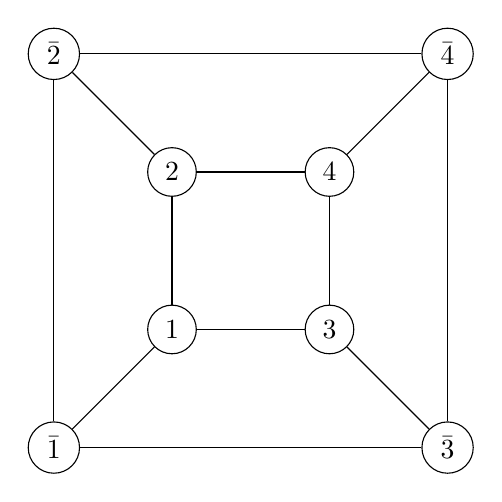
\begin{tikzpicture}
\node[circle,draw] (1b) {$\bar 1$};
\node[circle,draw] (2b) at (0,5) {$\bar 2$};
\node[circle,draw] (3b) at (5,0) {$\bar 3$};
\node[circle,draw] (4b) at (5,5) {$\bar 4$};

\node[circle,draw] (1) at (1.5,1.5) {$1$};
\node[circle,draw] (2) at (1.5,3.5) {$2$};
\node[circle,draw] (3) at (3.5,1.5) {$3$};
\node[circle,draw] (4) at (3.5,3.5) {$4$};

\draw (1b) edge (3b);
\draw (1b) edge (2b);
\draw (2b) edge (4b);
\draw (3b) edge (4b);
\draw (1) edge (3);
\draw (1) edge (2);
\draw (2) edge (4);
\draw (3) edge (4);
\draw (1) edge (1b);
\draw (2) edge (2b);
\draw (3) edge (3b);
\draw (4) edge (4b);
\end{tikzpicture}
\qquad
\tikz{
	\draw[->] (0,0) -- (2,0) node[midway,sloped,below]{ASI};
	\draw[->] (0,0) -- (0,2) node[midway,above,sloped]{ADF};
	\draw[->] (0,0) -- (-1.2,-1.2) node[midway,sloped,below]{NSM};
}

\vspace{.5cm}
\begin{tabular}{|c|c|c|c|}
\hline
state & ADF & ASI & NSM \\
\hline
1     & 0   & 0   & 0   \\
2     & 1   & 0   & 0   \\
3     & 0   & 1   & 0   \\
4     & 1   & 1   & 0   \\
$\bar 1$     & 0   & 0   & 1   \\
$\bar 2$     & 1   & 0   & 0   \\
$\bar 3$     & 0   & 1   & 0   \\
$\bar 4$     & 1   & 1   & 0   \\
\hline
\end{tabular}
\end{center}

The transition rate matrix is
\begin{equation}
W  =\left(\begin{array}{c c c c c c c c}
        -3k_{on}      & w_{xx}          & w_{yy}          & 0                               & w_{zz}          & 0                                 & 0                                 & 0\\
        k_{on}        & -2k_{on}-w_{xx} & 0               & w_{xy}w_{yy}                    & 0               & w_{xz}w_{zz}                      & 0                                 & 0\\
		k_{on}        & 0               & -w_{yy}-2k_{on} & w_{yx}w_{xx}                    & 0               & 0                                 & w_{yz}w_{zz}                      & 0\\
		0             & k_{on}          & k_{on}          & -k_{on}-w_{xx}w_{yx}-w_{yy}w_{xy} & 0               & 0                                 & 0                                 & w_{xz}w_{yz}w_{zz}\\
		k_{on}        & 0               & 0               & 0                               & -w_{zz}-2k_{on} & w_{zx}w_{xx}                      & w_{zy}w_{yy}                      & 0\\      
		0             & k_{on}          & 0               & 0                               & k_{on}          & -k_{on}-w_{zx}w_{xx}-w_{xz}w_{zz} & 0                                 & w_{yy}w_{xy}w_{zy}\\      
		0             & 0               & k_{on}          & 0                               & k_{on}          & 0                                 & -w_{zz}w_{yz}-w_{yy}w_{zy}-k_{on} & w_{xx}w_{yx}w_{zx}\\      
		0             & 0               & 0               & k_{on}                          & 0               & k_{on}                            & k_{on}                            & -w_{zz}w_{xz}w_{yz}-w_{xx}w_{yx}w_{zx}-w_{yy}w_{xy}w_{zy}     
		\end{array}
  \right)
\end{equation}

To access the parameters of the regulatory matrix $R={w_{ij}}$ I used the notation
\begin{equation}
R=\left( \begin{array}{c c c}
             w_{xx} & w_{xy} & w_{xz} \\
             w_{yx} & w_{yy} & w_{yz} \\
             w_{zx} & w_{zy} & w_{zz} 
	     \end{array} \right) = 
  \left( \begin{array}{c c c}
             t_1 & t_2 & t_3\\
			 t_4 & t_5 & t_6\\
			 t_7 & t_8 & t_9
	     \end{array}\right)
 \end{equation}
\end{document}
